% LuxSleek-CV 1.1 LaTeX template
% Author: Andreï V. Kostyrka, University of Luxembourg
%
% 1.1: added tracking and letter-spacing for prettier lower caps, added `~` for language levels
% 1.0: initial release
%
% This template fills the gap in the available variety of templates
% by proposing something that is not a custom class, not using any
% hard-coded settings deeply hidden in style files, and provides
% a handful of custom command definitions that are as transparent as it gets.
% Developed at the University of Luxembourg.
%
% *NOTHING IS HARCODED, and never should be.*
%
% Target audience: applicants in the IT industry, or business in general
%
% The main strength of this template is, it explicitly showcases how
% to break the flow of text to achieve the most flexible right alignment
% of dates for multiple configurations.

\documentclass[11pt, letterpaper]{article} 
\usepackage{fontawesome}
\usepackage[T1]{fontenc}     % We are using pdfLaTeX,
\usepackage[utf8]{inputenc}  % hence this preparation
\usepackage[british]{babel}  
\usepackage[left = 0mm, right = 0mm, top = 0mm, bottom = 0mm]{geometry}
\usepackage[stretch = 25, shrink = 25, tracking=true, letterspace=30]{microtype}  
\usepackage{graphicx}        % To insert pictures
\usepackage{xcolor}          % To add colour to the document
\usepackage{tikz}
\usetikzlibrary{arrows.meta, positioning, calc}

\usepackage{enumitem}        % To redefine spacing in lists
\setlist{parsep = 0pt, topsep = 0pt, partopsep = 1pt, itemsep = 1pt, leftmargin = 6mm}

\usepackage[sfdefault]{FiraSans} % Change this to use any font, but keep it simple

\definecolor{cvblue}{HTML}{304263}

%%%%%%% USER COMMAND DEFINITIONS %%%%%%%%%%%%%%%%%%%%%%%%%%%
% These are the real workhorses of this template
\newcommand{\experienceitem}[3]{%
\is
\textsc{\textbf{#1}} at \textit{#2}\hfill\mbox{\textit{#3}} \\
}
\newcommand{\is}{\par\vskip.5ex plus .4ex} % Item spacing
\newcommand{\achievement}[2]{{\small\raisebox{-0.2ex}{\tikz[remember picture]\node[] (#1) {$\diamond$};}#2}}
\newcommand{\headleft}[1]{\vspace*{3ex}\textsc{\textbf{#1}}\par%
    \vspace*{-1.5ex}\hrulefill\par\vspace*{0.7ex}}
\newcommand{\headright}[1]{\vspace*{2.5ex}\textsc{\Large\color{cvblue}#1}\par%
     \vspace*{-2ex}{\color{cvblue}\hrulefill}\par}
\newenvironment{experience}{%
   \headright{Experience}
   \vspace*{-.9ex}
}{}
\newenvironment{skills}{%
  \headleft{Skills}
  \vspace*{0.4ex}
  \small
  \raggedleft
}{%
}
\newcommand{\skill}[3]{%
  \raisebox{0.4ex}{#3}\tikz[remember picture]\node[] (#2) {\color{#1}$\bullet$};\\
}
%%%%%%%%%%%%%%%%%%%%%%%%%%%%%%%%%%%%%%%%%%%%%%%%%%%%%%%%%%%%

\usepackage[colorlinks = true, urlcolor = white, linkcolor = white]{hyperref}

% Style definitions -- killing the unnecessary space and adding the skips explicitly
\setlength{\topskip}{0pt}
\setlength{\parindent}{0pt}
\setlength{\parskip}{0pt}
\setlength{\fboxsep}{0pt}
\pagestyle{empty}

\begin{document}%
\raggedbottom

\begin{minipage}[t]{0.33\textwidth} %% Left column -- outer definition
%  Left column -- top dark rectangle
\colorbox{cvblue}{\begin{minipage}[t][5mm][t]{\textwidth}\null\hfill\null\end{minipage}}%

\vspace{-.25ex}% Eliminates the small gap
\colorbox{cvblue!90}{\color{white}  %% LEFT BOX
\kern0.09\textwidth\relax% Left margin provided explicitly
\begin{minipage}[t][\dimexpr\textheight-5mm\relax][t]{0.82\textwidth}
\raggedright
\vspace*{2.5ex}

\null\hfill\Huge{Jason \textbf{\textsc{Felice,}}}\normalsize\hfill\null

% Centering without extra vertical spacing
\null\hfill
\includegraphics[width=0.65\textwidth]{profile.jpg}\hfill\null

\vspace*{0.5ex} % Extra space after the picture
{\small
 a business focused, collaborative, hands-on, multi-language tech lead, architect, and large system builder.
}

\headleft{Count on me to}
{\small
 create sustainable software, bring all voices to the process, facilitate and mentor, embody compassion, and use the best of Agile/XP.
}

\begin{skills}
\skill{red}{writing}{Written Communication}
\skill{cyan}{broadbrief}{Broad Brief}
\skill{green}{inceptiontocompletion}{Inception to Completion}
\skill{orange}{cicd}{CI/CD}
\skill{blue}{react}{React}
\skill{violet}{nodejs}{Node.js}
\skill{magenta}{production}{Large Scale/Production}
\skill{olive}{mysql}{MySQL}
\end{skills}

\headleft{Interests}
{\small systems \textbullet\ emergence \textbullet\ geek joy \\
making \textbullet\ nonviolent communication \\
math \textbullet\ data \textbullet\ algorithms \\
open source software \\
}\normalsize

\vfill
\headleft{Contact}
\makebox[1em][c]{\faAt}\ jason.m.felice@gmail.com \\[0.5ex]
\makebox[1em][c]{\faPhone}\ +1\,216\,466\,4122 \\[0.5ex]
\makebox[1em][c]{\faGithub}\ \href{https://github.com/eraserhd}{github.com/eraserhd} \\[0.5ex]
\makebox[1em][c]{\faCode}\ \href{https://www.topcoder.com/members/eraserhd}{topcoder.com/eraserhd} \\[0.5ex]
\makebox[1em][c]{\faMapMarker}\ Euclid, Ohio, USA\\
\vspace*{5ex}

\end{minipage}%
\kern0.09\textwidth\relax%%Right margin provided explicitly to stretch the colourbox
}%
\end{minipage}% Right column
\hskip2.5em% Left margin for the white area
\begin{minipage}[t]{0.56\textwidth}

\setlength{\parskip}{0.8ex}% Adds spaces between paragraphs; use \\ to add new lines without this space. Shrink this amount to fit more data vertically

\vspace{2ex}

\vskip1.25ex
\headright{Large System Builder}
\vspace*{-2ex}
\null\hfill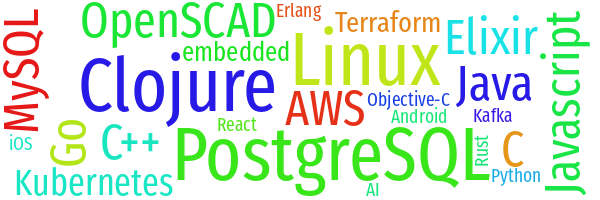
\includegraphics[width=0.95\textwidth]{techwords.png}\hfill\null
\vspace*{-2ex}


\begin{experience}
\experienceitem{Software Engineer IV}{2U}{2016--2025}
\achievement{centralpark}{Automated new program standup} \\
\achievement{nexus}{Brought an acquired company's tech stack up to 2U standards} \\
\achievement{coresystems}{Maintained core systems and influenced technical direction}

\experienceitem{Software Engineer IV}{Groupon}{2013--2016}
\achievement{homepage}{Implemented and delivered new homepage} \\
\achievement{points}{Designed and delivered Points retention program} \\
\achievement{whitepaper}{Broke a delivery-limiting stalemate between tech and purchasing}

\experienceitem{iOS \& Android Developer}{LeanDog}{2011--2013}
\achievement{eriemobile}{Maintained iOS application and ported it to Android}

\experienceitem{Software Engineer}{Blue Frog Gaming}{2010--2011}
\achievement{polarpuzzles}{Designed and delivered Polar Puzzles and Ghost Chicken iPad games} \\
\achievement{hearts}{Maintained Hearts and Spades iPad games and network servers}

\experienceitem{Senior Software Engineer}{Micros Retail}{2007--2010}
\achievement{xpay}{Maintained DAS and XPay credit authorization systems} \\
\achievement{kanban}{Implemented processes dramatically reducing delivery failures}

\experienceitem{Chief Technology Officer}{Cronosys, LLC}{2000--2007}
\achievement{webtech}{Made a bet on web technology for internal business apps} \\
\achievement{cronosysprojects}{Consulted, quoted, and delivered many projects on many tech stacks}

\experienceitem{Consultant}{The Baldwin Group}{1997--2000}
\achievement{pcconsulting}{Consulted on PC-related issues} \\
\achievement{mayorscourt}{Maintained Mayor's Court software}

\experienceitem{Programmer/Analyst}{DataVantage}{1994--1997}
\achievement{datacomm}{Automated third shift data communications} \\
\achievement{auth21}{Implemented new credit authorization system} \\
\achievement{instoreplus}{Maintained point-of-sale software}
\end{experience}%
\end{minipage}%
\begin{tikzpicture}[remember picture, overlay,
                    -Stealth, thick,
                    white!60!black,
                    rounded corners]
    \draw [red] (writing) -- ++(0.3,0) |- (whitepaper);
    \draw [cyan] (broadbrief) -- ++(0.45,0) |- (centralpark);
    \draw [cyan] (broadbrief) -- ++(0.45,0) |- (points);
    \draw [cyan] (broadbrief) -- ++(0.45,0) |- (datacomm);
    \draw [cyan] (broadbrief) -- ++(0.45,0) |- (auth21);
    \draw [cyan] (broadbrief) -- ++(0.45,0) |- (cronosysprojects);
    \draw [green] (inceptiontocompletion) -- ++(0.6,0) |- (centralpark);
    \draw [green] (inceptiontocompletion) -- ++(0.6,0) |- (points);
    \draw [green] (inceptiontocompletion) -- ++(0.6,0) |- (homepage);
    \draw [green] (inceptiontocompletion) -- ++(0.6,0) |- (datacomm);
    \draw [green] (inceptiontocompletion) -- ++(0.6,0) |- (auth21);
    \draw [green] (inceptiontocompletion) -- ++(0.6,0) |- (polarpuzzles);
    \draw [green] (inceptiontocompletion) -- ++(0.6,0) |- (cronosysprojects);
    \draw [orange] (cicd) -- ++(0.75,0) |- (nexus);
    \draw [orange] (cicd) -- ++(0.75,0) |- (kanban);
    \draw [blue] (react) -- ++(0.95,0) |- (nexus);
    \draw [blue] (react) -- ++(0.95,0) |- (centralpark);
    \draw [violet] (nodejs) -- ++(1.1,0) |- (coresystems);
    \draw [violet] (nodejs) -- ++(1.1,0) |- (homepage);
    \draw [magenta] (production) -- ++(1.25,0) |- (points);
    \draw [magenta] (production) -- ++(1.25,0) |- (xpay);
    \draw [olive] (mysql) -- ++(1.4,0) |- (coresystems);
    \draw [olive] (mysql) -- ++(1.4,0) |- (cronosysprojects);
\end{tikzpicture}%
\end{document}
